\subsection{Acapulco (Mexican Original)}
\vspace{-7.5mm}
\hspace{71mm}
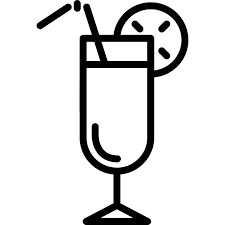
\includegraphics[scale=.07]{cocktail_glass_tall.png}
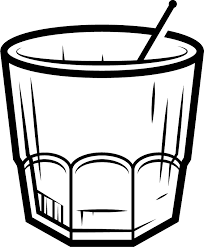
\includegraphics[scale=.06]{cocktail_glass_rock.png}
\vspace{2.5mm}
\begin{itembox}[l]{\boldmath $\reci$}
\begin{itemize}
\setlength{\parskip}{0cm}
\setlength{\itemsep}{0cm}
\item \teq 30ml
\item \rum 30ml
\item \pj 24ml
\item \gj 15ml
\item \limj 15ml
\item \sugar (or \gumsyrup) 2tsp
\end{itemize}
\vspace{-4mm}
Made by \shake
\end{itembox}
The Acapulco cocktail is the beautiful love child of a Hemingway Daiquiri and a Margarita.
%%Originally from (you guessed it) Acapulco, Mexico
%%, it's made with both tequila and rum as well as a fruity mix of lime, pineapple and grapefruit juice.
%If you're looking for the perfect summertime libation, look no further. 
